\section{Phase 1: Input Parameter Tuning for Output Quality}
\label{phase1}

\subsection{Goal}
Phase 1 of the experiments seeks to quantify the effects of running the system with different combinations of input parameters. The reasons for this are twofold:

\begin{enumerate}
\item Firstly, it grounds these esoteric parameters \gls{error rate} limit (\bfit{e}) and prefix length threshold (\bfit{t}) in reality, allowing the user to gain an understanding of how to get the most out of the solver.

\item Secondly, it allows the experiments in Phase 2 and Phase 3 the assumption of a constrained possibility space. Assuming users are after high \textit{quality} output solutions with respect to the expected use case, it becomes possible to affix \bfit{t} and \bfit{e}; This allows more targeted testing and optimization such that the system achieves optimal speed specifically for these expected use cases.
\end{enumerate}

\subsection{Experimental Design}
Our definition of \textit{output quality} is based on \textit{F-measure}\footnote{$\text{\textit{F-measure}} = 2 \cdot{} precision \cdot{} recall / (precision + recall)$} which seeks to incorporate precision and recall; Counts for \textit{true positive}, \textit{false positive} etc. are  defined with respect to \glspl{solution} from a predetermined \textit{ground truth} solution set, which is the set of overlaps whose strings really do come from overlapping regions of the \gls{source genome}. To approximate a realistic instance of such true solutions, the data set is constructed from simulated reads from a \textit{real} genome sequence of an HIV-1 reference strain (HXB2), introducing errors according to an \textit{error profile} designed to model the physical nucleotide-reading process. In our case, the ground truth set consists of 4,854,458 unique overlap \glspl{solution}.

High recall is desirable for sequence assembly, as it directly corresponds with how effectively the system utilizes the \glspl{genome copy} of the \gls{source genome} (measured as data set \gls{coverage}). \textit{False negative} solutions reduce recall, and when used for sequence assembly, could potentially prevent the formation of a good overlap chain, and consequentially, result in a less-satisfactory assembly.

High precision is also desirable, as it reduces the run time of any tool that needs to filter out \textit{false positive} solutions. Some use cases might also find false positive overlaps undesirable, as they might negatively impact their own output quality or runtime.


\FloatBarrier

\subsection{Results}
The recall and precision of individual \aspop{} solver executions can be seen in Figure \ref{fig:phase1_plots}, with a 3D surface for recall, and another for precision; Figure \ref{fig:phase1_02} plots the corresponding values for f-measure. Throughout all surfaces, the same $(\bfit{t}, \bfit{e})$ coordinates correspond with the same execution's output set.


\begin{figure}
\centering
   \begin{subfigure}[b]{0.8\textwidth}
   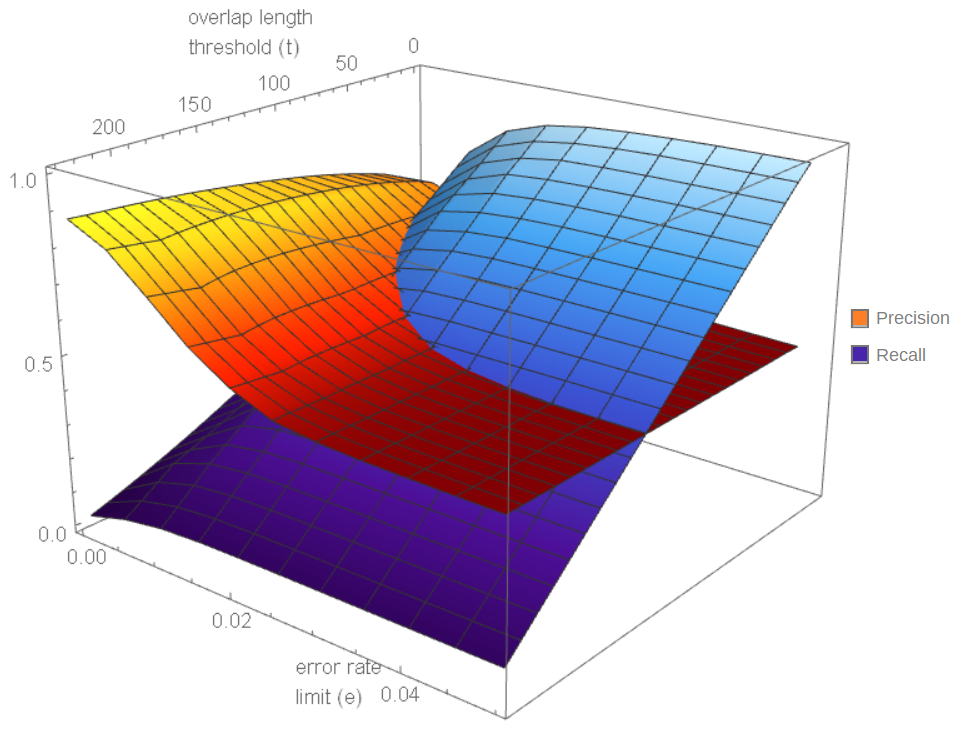
\includegraphics[width=1\linewidth]{images/phase1_A.png}
   \caption{}
\end{subfigure}

\begin{subfigure}[b]{0.8\textwidth}
   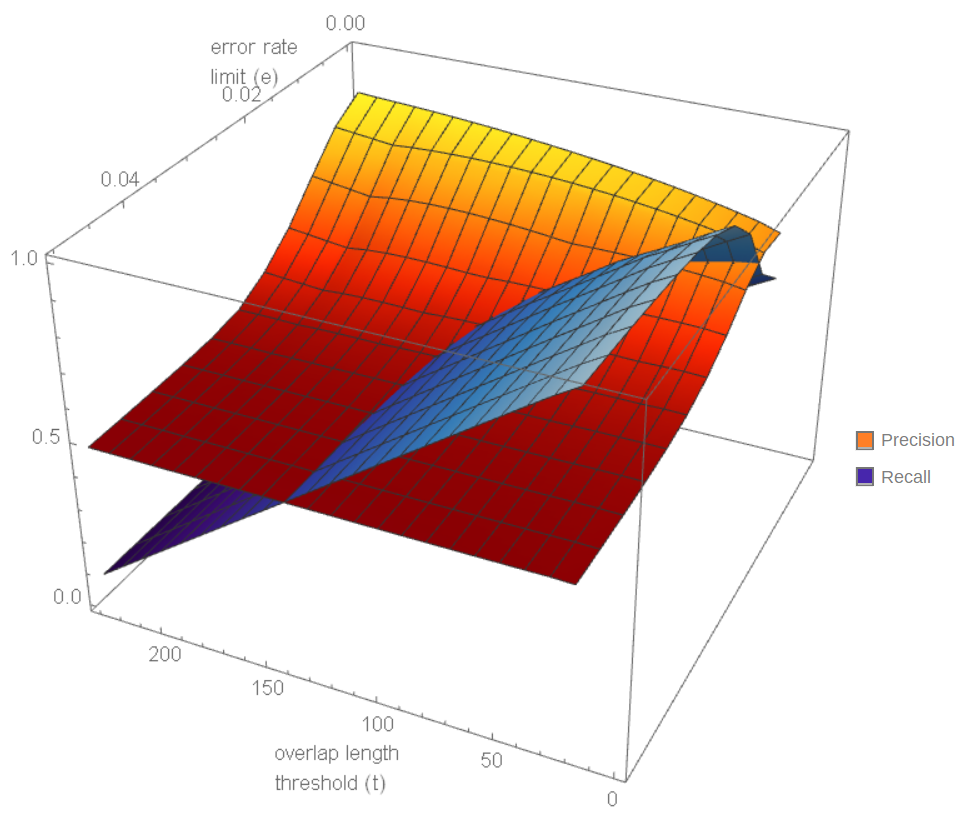
\includegraphics[width=1\linewidth]{images/phase1_B.png}
   \caption{}
\end{subfigure}

\caption[Precision and recall for output solution sets generated from runs using various \bfit{e} and \bfit{t} values.]{(a) Precision and recall for output solution sets generated from runs using various \bfit{e} and \bfit{t} values. (b) Alternative view.}
\label{fig:phase1_plots}
\end{figure}
\subsection{Observations}

As was expected, Figure \ref{fig:phase1_plots} shows that the solver achieves highest recall with restrictions relaxed as much as possible (low \bfit{t} and high \bfit{e}).

Outputs with the highest precision scores were the ones in which only \glspl{solution} \textit{highly} likely to be real were output.
\begin{enumerate}
\item Solutions that have longer overlaps are more likely to be real, explaining the correlation between high \bfit{t} and high precision.
\item Solutions that represent overlaps with very few errors are more likely to be real. Increased error blurs the distinction between different subsequences of the genome, increasing the number of false positives.
\end{enumerate}

Beyond approximately 3\% error, not much seems to change with respect to either metric, as can be seen in the `plateauing' of both recall and precision surfaces.

Clearly there is a trade-off between recall and precision to be considered when selecting one's input parameters. As very low values for either are highly undesirable, the values for run \textit{F-measures} in figure \ref{fig:phase1_02} give a view of the relative \textit{quality} of each run, factoring in the contributions of both recall and precision.


\begin{figure}[!htb]
\centering
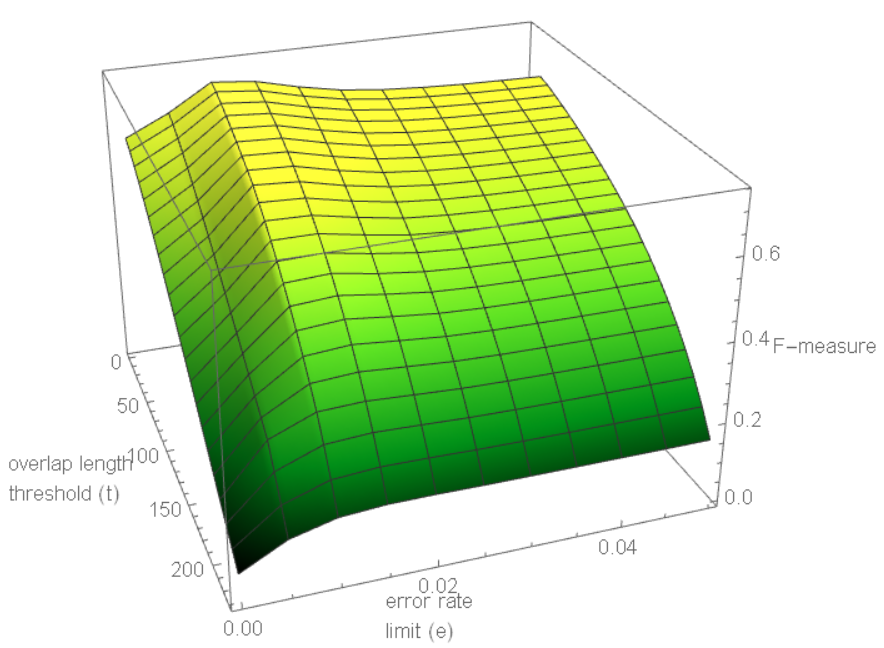
\includegraphics[width=0.9\textwidth]{images/fmeasure.png}
\caption{F-measure of output solution sets generated from runs using various \bfit{e} (error rate limit) and \bfit{t} (overlap threshold length) values.}
\label{fig:phase1_02}
\end{figure}

Use of shorter \bfit{t} appears to be consistently beneficial, and the choice of \bfit{e} seems optimal at approximately 1.2\% regardless of \bfit{t}. As exceptionally short overlap threshold of $< 80$ is undesirable for sequence assembly of viral genomes\footnote{See Section \ref{context} for more information on this choice of threshold.} (our primary use case), the optimal choice of parameters seems to be:
\begin{align*}
\bfit{t} &= 80\\
\bfit{e} &= 1.2\%
\end{align*}

\FloatBarrier
